
\documentclass[a4paper, 12pt, finnish]{article}

\usepackage{babel}
\usepackage[utf8]{inputenc}
\usepackage[T1]{fontenc}
\usepackage{amsmath}
\usepackage{graphicx}
\usepackage{hyperref}

\title{Muistilistan dokumentaatio}

\author{Ossi Räisä}

\begin{document}

\maketitle

\section{Johdanto}

Muistilistan on tarkoitus auttaa käyttääjää muistamaan kaikki hänelle annetut tehtävät.
Jokainen tehtävä lisätään listaan. Tehtävään kuuluu lyhyt kuvaus, tärkeys, ja mahdollisesti
deadline. Tehtäville voi myös antaa tägin. Tägit periytyvät, eli jokaisella tägillä voi olla
yksi tai useampia vanhempia. Käyttäjä voi hakea omia tehtäviään tägien ja tärkeyden perusteella
ja järjestää tuloksia tärkeyden perusteella. Tehtävän voi poistaa tai merkitä suoritetuksi.
Tehtäviä ja tägejä voi myös muokata jälkeenpäin. Käyttäjien täytyy kirjautua sisään käyttätunnuksella
ja salasanalla.

Muistilista pyörii tietojenkäsittelytieteen laitoksen users-palvelimella ja käyttää php:tä
palvelimen logiikan toteuttamiseen. Käyttöliittymä käyttää javascriptiä, jos se on tarpeen.
Tehtävät ja käyttäjien tiedot tallennetaan PostgreSQL-tietokantaan.

\newpage

\section{Käyttötapaukset}

\begin{figure}[h]
  \caption{Käyttötapauskaavio}
  \centering
  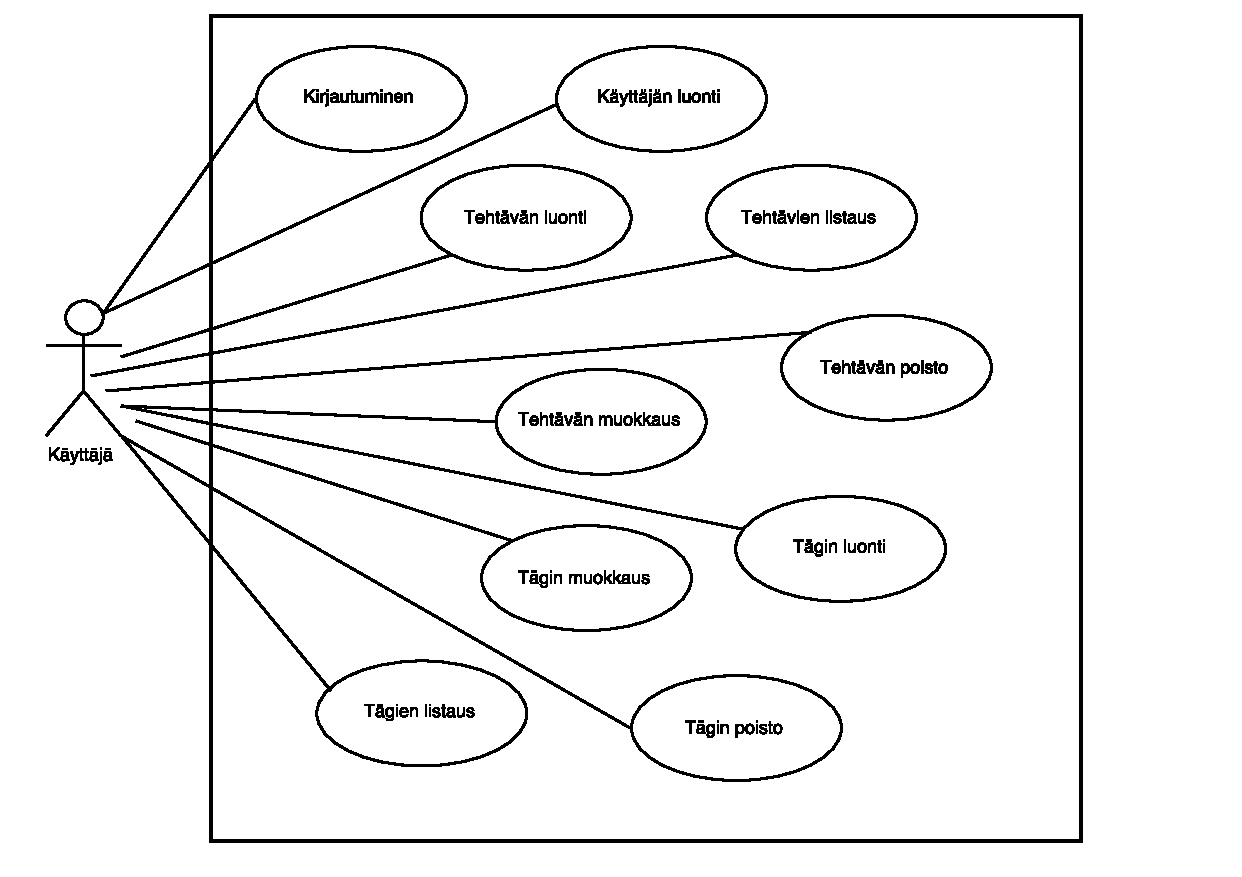
\includegraphics[scale=0.7]{kayttotapauskaavio}
\end{figure}

\subsection{Käyttötapauksien kuvauksia}
\begin{description}
  \item[Tehtävän luonti] \hfill \\
  Tehtävää luodessa käyttäjä voi asettaa tehtävälle tärkeyden, antaa kuvauksen,
  asettaa deadlinen ja antaa tehtävälle tägin.
  \item[Tehtävien listaus] \hfill \\
  Käyttäjä voi listata kaikki tehtävät tai rajata listausta tehtävien tärkeyden,
  deadlinen (kaikki joissa deadline ennen), ja tägien perusteella (kaikki joilla tietty
  tägi tai jokin sen lapsista).
  \item[Tägin luonti] \hfill \\
  Tägin voi luoda uutta tehtävää luodessa, jos uudelle tägille on tarvetta tai
  pääsivulta. Tägiä luodessa käyttäjä antaa nimen sekä mahdolliset vanhemmat.
  Tägiä luodessa on myös mahdollista luoda uusi vanhempi.
  \item[Muita käyttötapauksia] \hfill \\
  Tehtävää tai tägiä muokkaamaan pääsee listaussivulta ja kaikkea, mitä luodessa
  voi asettaa voi muokata. Poisto tapahtuu muokkaussivulta.
\end{description}

\section{Järjestelmän tietosisältö}

\begin{figure}[h]
  \caption{Käsitekaavio}
  \centering
  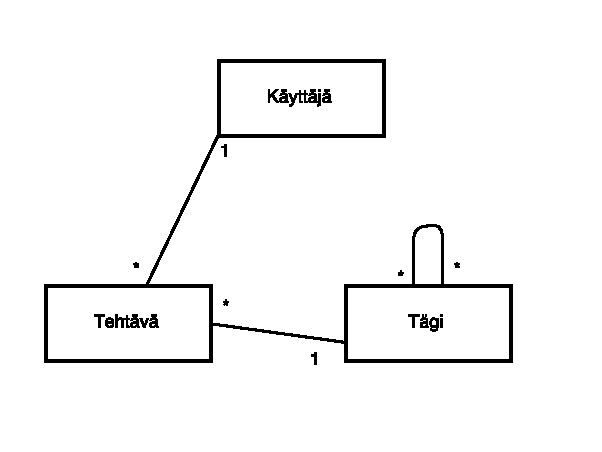
\includegraphics[scale=1.0]{kasitekaavio}
\end{figure}

\subsection{User}
\begin{tabular}{l | l | l}
  Attribuutti & Arvojoukko \\ \hline
  username & merkkijono (50 merkkiä) \\ \hline
  password & merkkijono (50 merkkiä) \\
\end{tabular}
\\
User-tauluun tallennetaan jokaisen käyttäjän kirjautumistiedot

\subsection{Assingment}
\begin{tabular}{l | l | l}
  Attribuutti & Arvojoukko \\ \hline
  name & merkkijono (50 merkkiä) \\ \hline
  importance & kokonaisluku \\ \hline
  deadline & päivämäärä ja aika \\ \hline
  description & merkkijono (500 merkkiä) \\
\end{tabular}
\\
Assingment-tauluun tallennetaan tehtävät. Kaikilla tehtävillä on omistaja, joka
on tehtävän luonut käyttäjä. Tehtävillä voi myös olla yksi tägi.
Deadline-sarake käyttää SQL:n datetime-tyyppiä.

\subsection{Tag}
\begin{tabular}{l | l | l}
  Attribuutti & Arvojoukko \\ \hline
  name & merkkijono (50 merkkiä) \\
\end{tabular}
\\
Tägeillä on nimi ja niillä voi myös olla ylätägejä. Tägin perusteella haettaessa
myös tägin lapsilla merkatut tehtävät sisältyvät tuloksiin.

\section{Relaatiotietokantakaavio}

\begin{figure}[h]
  \caption{Tietokantakaavio}
  \centering
  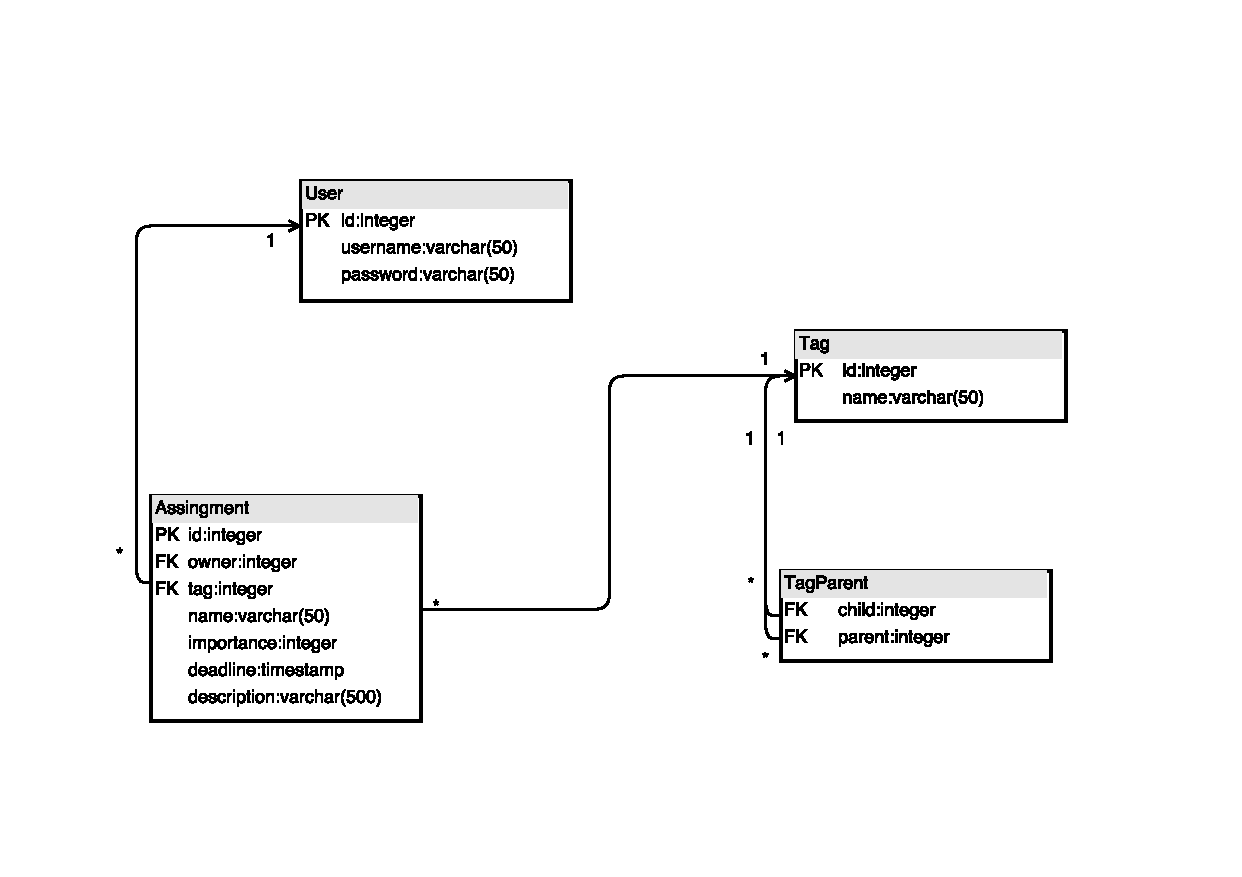
\includegraphics[scale=0.7]{tietokantakaavio}
\end{figure}

Huom: Tag-taululla on myös owner-attribuutti kuten Assignment-taululla.

\section{Järjestelmän yleisrakenne}
Muistilista on tehty MVC-mallin mukaisesti. Mallit sijaitsevat kansiossa src/models,
näkymät kansiossa src/views ja kontrollerit kansiossa src/controllers. Lisäksi src/routes.php
sisältää sovelluksen reitit ja src/db.php sisältää tietokannan avaamisen. Sovelluksen käyttämät
kirjastot ovat lib-kansiossa.

\section{Käyttöliittynä ja järjestelmän komponentit}

\begin{figure}[h]
  \caption{Käyttöliittymä}
  \centering
  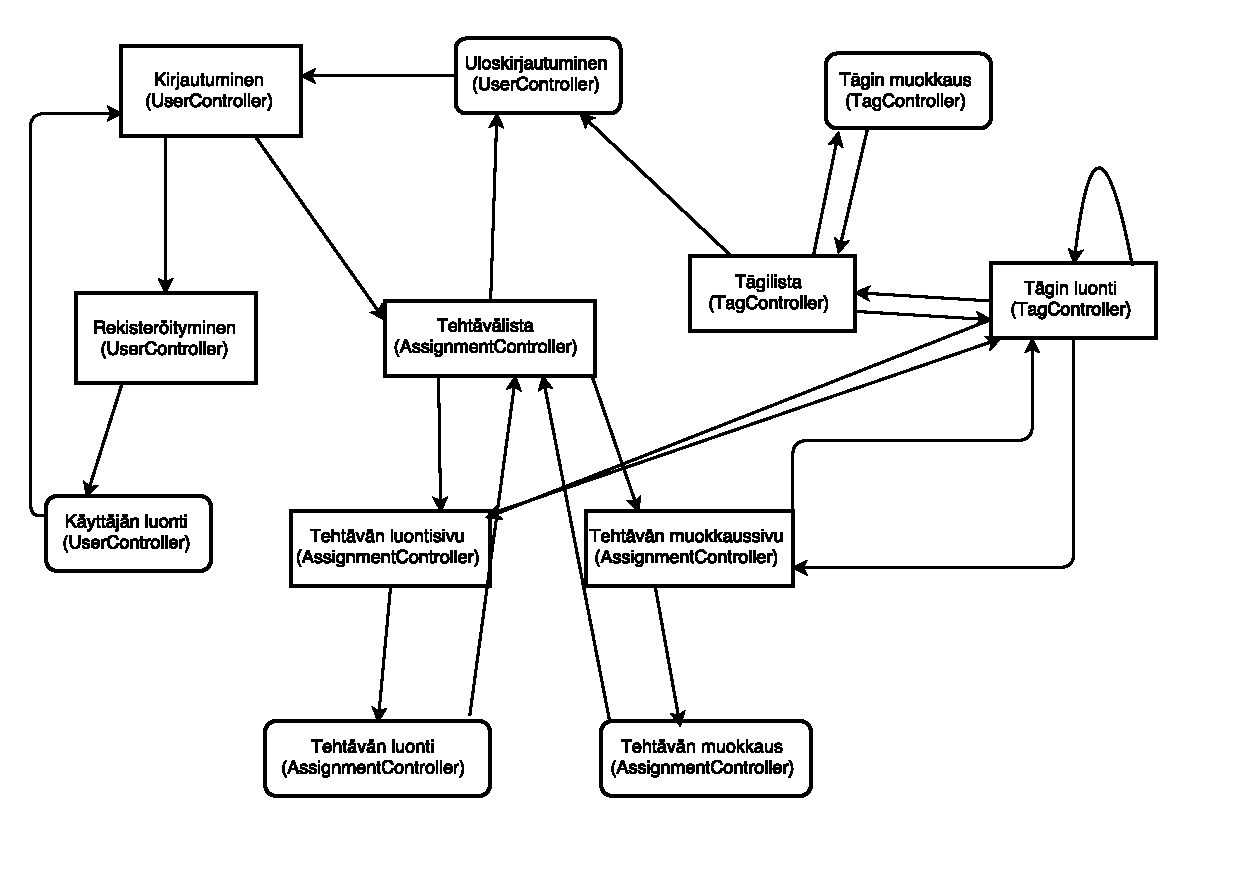
\includegraphics[scale=0.6]{kayttoliittyma}
\end{figure}
Kaikki sivut kirjautumista ja rekisteröitymistä lukuun ottamatta vaativat kirjautumisen.

\section{Asennusohje}
Muistilistan voi asentaa suorittamalla deploy.sh-tiedoston, kunhan deploy.sh-tiedostoon on laitettu
kohdepalvelimen osoite oikein. Sovelluksen täytyy olla muitilista-nimisessä kansiossa. Käytettäessä jotain
muuta tietokantaa kuin PostgreSQL:ä db.php-tiedostoa täytyy muokata niin, että tietokantayhteys muodostetaan
oikeaan tietokannanhallintajärjestelmään. Tietokanta täytyy alustaa suorittamalla src/sql-kansiossa olevat
tiedostot valitulla tietokannanhallintajärjestelmällä. add\_test\_data.sql-tiedostoa ei tarvitse suorittaa, jos
testidataa ei haluta lisätä tietokantaan.

\section{Käynnistys- ja käyttöohje}

\href{https://oraisa.users.cs.helsinki.fi/muistilista}{Kirjautumissivu} \\
\begin{description}
  \item[Testikäyttäjät] \hfill \\
  testi, salasana 1234 \\
  testi2, salasana password
\end{description}

\end{document}
